\documentclass{ximera}
%
%%% Begin Laad packages
%
\makeatletter
\@ifclassloaded{xourse}{%
    \typeout{Start loading preamble.tex (in a XOURSE)}%
    \def\isXourse{true}   % automatically defined; pre 112022 it had to be set 'manually' in a xourse
}{%
    \typeout{Start loading preamble.tex (NOT in a XOURSE)}%
}
\makeatother

\pgfplotsset{compat=1.16}

\usepackage{currfile}

% 201908/202301: PAS OP: babel en doclicense lijken problemen te veroorzaken in .jax bestand
% (wegens syntax error met toegevoegde \newcommands ...)
\pdfOnly{
    \usepackage[hyperxmp=false,type={CC},modifier={by-nc-sa},version={4.0}]{doclicense}
    \usepackage[dutch]{babel}
}


\usepackage[utf8]{inputenc}
\usepackage{morewrites}   % nav zomercursus (answer...?)
\usepackage{multirow}
\usepackage{multicol}
\usepackage{tikzsymbols}
\usepackage{tikz-3dplot}
\usepackage{ifthen}
%\usepackage{animate} BREAKS HTML STRUCTURE USED BY XIMERA
\usepackage{relsize}

\usepackage{eurosym}    % \euro  (€ werkt niet in xake ...?)
\usepackage{wrapfig}

\usepackage{cancel}

\usepackage{tabularx}
% Nuttig als ook interactieve beamer slides worden voorzien:
\providecommand{\p}{} % default nothing ; potentially usefull for slides: redefine as \pause
%providecommand{\p}{\pause}

\usepackage{caption} % captionof
%\usepackage{pdflscape}    % landscape environment

% Met "\newcommand\showtodonotes{}" kan je todonotes tonen (in pdf/online)
% 201908: online werkt het niet (goed)
\providecommand\showtodonotes{disable}
\providecommand\todo[1]{\typeout{TODO #1}}
%\usepackage[\showtodonotes]{todonotes}
%\usepackage{todonotes}

%
% Poging tot aanpassen layout
%
\usepackage{tcolorbox}
\tcbuselibrary{theorems}

%%% Einde laad packages

%%% Begin Ximera specifieke zaken

% \graphicspath{
% 	{../../}
% 	{../}
% 	{./}
%   	{../../pictures/}
%    	{../pictures/}
%    	{./pictures/}
% 	{./explog/}    % M05 in groeimodellen       
% }

%%% Einde Ximera specifieke zaken

%
% define softer blue/red/green, use KU Leuven base colors for blue (and dark orange for red ?)
%
% todo: rather redefine blue/red/green ...?
%\definecolor{xmblue}{rgb}{0.01, 0.31, 0.59}
%\definecolor{xmred}{rgb}{0.89, 0.02, 0.17}
\definecolor{xmdarkblue}{rgb}{0.122, 0.671, 0.835}   % KU Leuven Blauw
\definecolor{xmblue}{rgb}{0.114, 0.553, 0.69}        % KU Leuven Blauw
\definecolor{xmgreen}{rgb}{0.13, 0.55, 0.13}         % No KULeuven variant for green found ...

\definecolor{xmaccent}{rgb}{0.867, 0.541, 0.18}      % KU Leuven Accent (orange ...)
\definecolor{kuaccent}{rgb}{0.867, 0.541, 0.18}      % KU Leuven Accent (orange ...)

\colorlet{xmred}{xmaccent!50!black}                  % Darker version of KU Leuven Accent

\providecommand{\blue}[1]{{\color{blue}#1}}    
\providecommand{\red}[1]{{\color{red}#1}}

\renewcommand\CancelColor{\color{xmaccent!50!black}}

% werkt in math en text mode om MATH met oranje (of grijze...)  achtergond te tonen (ook \important{\text{blabla}} lijkt te werken)
%\newcommand{\important}[1]{\ensuremath{\colorbox{xmaccent!50!white}{$#1$}}}   % werkt niet in Mathjax
%\newcommand{\important}[1]{\ensuremath{\colorbox{lightgray}{$#1$}}}
%\newcommand{\important}[1]{\ensuremath{\colorbox{orange}{$#1$}}}   % TODO: kleur aanpassen voor mathjax; wordt overschreven infra!
\newcommand{\important}[1]{\ensuremath{\fcolorbox{black}{white}{$#1$}}}


% Uitzonderlijk kan met \pdfnl in de PDF een newline worden geforceerd, die online niet nodig/nuttig is omdat daar de regellengte hoe dan ook niet gekend is.
\ifdefined\HCode%
\providecommand{\pdfnl}{}%
\else%
\providecommand{\pdfnl}{%
  \\%
}%
\fi

% Uitzonderlijk kan met \handoutnl in de handout-PDF een newline worden geforceerd, die noch online noch in de PDF-met-antwoorden nuttig is.
\ifdefined\HCode
\providecommand{\handoutnl}{}
\else
\providecommand{\handoutnl}{%
\ifhandout%
  \nl%
\fi%
}
\fi



% \cellcolor IGNORED by tex4ht ?
% \begin{center} seems not to wordk
    % (missing margin-left: auto;   on tabular-inside-center ???)
%\newcommand{\importantcell}[1]{\ensuremath{\cellcolor{lightgray}#1}}  %  in tabular; usablility to be checked
\providecommand{\importantcell}[1]{\ensuremath{#1}}     % no mathjax2 support for colloring array cells

\pdfOnly{
  \renewcommand{\important}[1]{\ensuremath{\colorbox{kuaccent!50!white}{$#1$}}}
  \renewcommand{\importantcell}[1]{\ensuremath{\cellcolor{kuaccent!40!white}#1}}   
}

%%% Tikz styles


\pgfplotsset{compat=1.16}

\usetikzlibrary{trees,positioning,arrows,fit,shapes,math,calc,decorations.markings,through,intersections,patterns,matrix}

\usetikzlibrary{decorations.pathreplacing,backgrounds}    % 5/2023: from experimental


\usetikzlibrary{angles,quotes}

\usepgfplotslibrary{fillbetween} % bepaalde_integraal
\usepgfplotslibrary{polar}    % oa voor poolcoordinaten.tex

\pgfplotsset{ownstyle/.style={axis lines = center, axis equal image, xlabel = $x$, ylabel = $y$, enlargelimits}} 

\pgfplotsset{
	plot/.style={no marks,samples=50}
}

\newcommand{\xmPlotsColor}{
	\pgfplotsset{
		plot1/.style={darkgray,no marks,samples=100},
		plot2/.style={lightgray,no marks,samples=100},
		plotresult/.style={blue,no marks,samples=100},
		plotblue/.style={blue,no marks,samples=100},
		plotred/.style={red,no marks,samples=100},
		plotgreen/.style={green,no marks,samples=100},
		plotpurple/.style={purple,no marks,samples=100}
	}
}
\newcommand{\xmPlotsBlackWhite}{
	\pgfplotsset{
		plot1/.style={black,loosely dashed,no marks,samples=100},
		plot2/.style={black,loosely dotted,no marks,samples=100},
		plotresult/.style={black,no marks,samples=100},
		plotblue/.style={black,no marks,samples=100},
		plotred/.style={black,dotted,no marks,samples=100},
		plotgreen/.style={black,dashed,no marks,samples=100},
		plotpurple/.style={black,dashdotted,no marks,samples=100}
	}
}


\newcommand{\xmPlotsColorAndStyle}{
	\pgfplotsset{
		plot1/.style={darkgray,no marks,samples=100},
		plot2/.style={lightgray,no marks,samples=100},
		plotresult/.style={blue,no marks,samples=100},
		plotblue/.style={xmblue,no marks,samples=100},
		plotred/.style={xmred,dashed,thick,no marks,samples=100},
		plotgreen/.style={xmgreen,dotted,very thick,no marks,samples=100},
		plotpurple/.style={purple,no marks,samples=100}
	}
}


%\iftikzexport
\xmPlotsColorAndStyle
%\else
%\xmPlotsBlackWhite
%\fi
%%%


%
% Om venndiagrammen te arceren ...
%
\makeatletter
\pgfdeclarepatternformonly[\hatchdistance,\hatchthickness]{north east hatch}% name
{\pgfqpoint{-1pt}{-1pt}}% below left
{\pgfqpoint{\hatchdistance}{\hatchdistance}}% above right
{\pgfpoint{\hatchdistance-1pt}{\hatchdistance-1pt}}%
{
	\pgfsetcolor{\tikz@pattern@color}
	\pgfsetlinewidth{\hatchthickness}
	\pgfpathmoveto{\pgfqpoint{0pt}{0pt}}
	\pgfpathlineto{\pgfqpoint{\hatchdistance}{\hatchdistance}}
	\pgfusepath{stroke}
}
\pgfdeclarepatternformonly[\hatchdistance,\hatchthickness]{north west hatch}% name
{\pgfqpoint{-\hatchthickness}{-\hatchthickness}}% below left
{\pgfqpoint{\hatchdistance+\hatchthickness}{\hatchdistance+\hatchthickness}}% above right
{\pgfpoint{\hatchdistance}{\hatchdistance}}%
{
	\pgfsetcolor{\tikz@pattern@color}
	\pgfsetlinewidth{\hatchthickness}
	\pgfpathmoveto{\pgfqpoint{\hatchdistance+\hatchthickness}{-\hatchthickness}}
	\pgfpathlineto{\pgfqpoint{-\hatchthickness}{\hatchdistance+\hatchthickness}}
	\pgfusepath{stroke}
}
%\makeatother

\tikzset{
    hatch distance/.store in=\hatchdistance,
    hatch distance=10pt,
    hatch thickness/.store in=\hatchthickness,
   	hatch thickness=2pt
}

\colorlet{circle edge}{black}
\colorlet{circle area}{blue!20}


\tikzset{
    filled/.style={fill=green!30, draw=circle edge, thick},
    arceerl/.style={pattern=north east hatch, pattern color=blue!50, draw=circle edge},
    arceerr/.style={pattern=north west hatch, pattern color=yellow!50, draw=circle edge},
    outline/.style={draw=circle edge, thick}
}




%%% Updaten commando's
\def\hoofding #1#2#3{\maketitle}     % OBSOLETE ??

% we willen (bijna) altijd \geqslant ipv \geq ...!
\newcommand{\geqnoslant}{\geq}
\renewcommand{\geq}{\geqslant}
\newcommand{\leqnoslant}{\leq}
\renewcommand{\leq}{\leqslant}

% Todo: (201908) waarom komt er (soms) underlined voor emph ...?
\renewcommand{\emph}[1]{\textit{#1}}

% API commando's

\newcommand{\ds}{\displaystyle}
\newcommand{\ts}{\textstyle}  % tegenhanger van \ds   (Ximera zet PER  DEFAULT \ds!)

% uit Zomercursus-macro's: 
\newcommand{\bron}[1]{\begin{scriptsize} \emph{#1} \end{scriptsize}}     % deprecated ...?


%definities nieuwe commando's - afkortingen veel gebruikte symbolen
\newcommand{\R}{\ensuremath{\mathbb{R}}}
\newcommand{\Rnul}{\ensuremath{\mathbb{R}_0}}
\newcommand{\Reen}{\ensuremath{\mathbb{R}\setminus\{1\}}}
\newcommand{\Rnuleen}{\ensuremath{\mathbb{R}\setminus\{0,1\}}}
\newcommand{\Rplus}{\ensuremath{\mathbb{R}^+}}
\newcommand{\Rmin}{\ensuremath{\mathbb{R}^-}}
\newcommand{\Rnulplus}{\ensuremath{\mathbb{R}_0^+}}
\newcommand{\Rnulmin}{\ensuremath{\mathbb{R}_0^-}}
\newcommand{\Rnuleenplus}{\ensuremath{\mathbb{R}^+\setminus\{0,1\}}}
\newcommand{\N}{\ensuremath{\mathbb{N}}}
\newcommand{\Nnul}{\ensuremath{\mathbb{N}_0}}
\newcommand{\Z}{\ensuremath{\mathbb{Z}}}
\newcommand{\Znul}{\ensuremath{\mathbb{Z}_0}}
\newcommand{\Zplus}{\ensuremath{\mathbb{Z}^+}}
\newcommand{\Zmin}{\ensuremath{\mathbb{Z}^-}}
\newcommand{\Znulplus}{\ensuremath{\mathbb{Z}_0^+}}
\newcommand{\Znulmin}{\ensuremath{\mathbb{Z}_0^-}}
\newcommand{\C}{\ensuremath{\mathbb{C}}}
\newcommand{\Cnul}{\ensuremath{\mathbb{C}_0}}
\newcommand{\Cplus}{\ensuremath{\mathbb{C}^+}}
\newcommand{\Cmin}{\ensuremath{\mathbb{C}^-}}
\newcommand{\Cnulplus}{\ensuremath{\mathbb{C}_0^+}}
\newcommand{\Cnulmin}{\ensuremath{\mathbb{C}_0^-}}
\newcommand{\Q}{\ensuremath{\mathbb{Q}}}
\newcommand{\Qnul}{\ensuremath{\mathbb{Q}_0}}
\newcommand{\Qplus}{\ensuremath{\mathbb{Q}^+}}
\newcommand{\Qmin}{\ensuremath{\mathbb{Q}^-}}
\newcommand{\Qnulplus}{\ensuremath{\mathbb{Q}_0^+}}
\newcommand{\Qnulmin}{\ensuremath{\mathbb{Q}_0^-}}

\newcommand{\perdef}{\overset{\mathrm{def}}{=}}
\newcommand{\pernot}{\overset{\mathrm{notatie}}{=}}
\newcommand\perinderdaad{\overset{!}{=}}     % voorlopig gebruikt in limietenrekenregels
\newcommand\perhaps{\overset{?}{=}}          % voorlopig gebruikt in limietenrekenregels

\newcommand{\degree}{^\circ}


\DeclareMathOperator{\dom}{dom}     % domein
\DeclareMathOperator{\codom}{codom} % codomein
\DeclareMathOperator{\bld}{bld}     % beeld
\DeclareMathOperator{\graf}{graf}   % grafiek
\DeclareMathOperator{\rico}{rico}   % richtingcoëfficient
\DeclareMathOperator{\co}{co}       % coordinaat
\DeclareMathOperator{\gr}{gr}       % graad

\newcommand{\func}[5]{\ensuremath{#1: #2 \rightarrow #3: #4 \mapsto #5}} % Easy to write a function


% Operators
\DeclareMathOperator{\bgsin}{bgsin}
\DeclareMathOperator{\bgcos}{bgcos}
\DeclareMathOperator{\bgtan}{bgtan}
\DeclareMathOperator{\bgcot}{bgcot}
\DeclareMathOperator{\bgsinh}{bgsinh}
\DeclareMathOperator{\bgcosh}{bgcosh}
\DeclareMathOperator{\bgtanh}{bgtanh}
\DeclareMathOperator{\bgcoth}{bgcoth}

% Oude \Bgsin etc deprecated: gebruik \bgsin, en herdefinieer dat als je Bgsin wil!
%\DeclareMathOperator{\cosec}{cosec}    % not used? gebruik \csc en herdefinieer

% operatoren voor differentialen: to be verified; 1/2020: inconsequent gebruik bij afgeleiden/integralen
\renewcommand{\d}{\mathrm{d}}
\newcommand{\dx}{\d x}
\newcommand{\dd}[1]{\frac{\mathrm{d}}{\mathrm{d}#1}}
\newcommand{\ddx}{\dd{x}}

% om in voorbeelden/oefeningen de notatie voor afgeleiden te kunnen kiezen
% Usage: \afg{(2\sin(x))}  (en wordt d/dx, of accent, of D )
% \afg kan evt al gedefinieerd zijn in xmPreamble, of overschreven worden  
\providecommand{\afg}[1]{\frac{\mathrm{d}}{\mathrm{d}x} \left(#1\right) }   % include in relevant exercises ...
% \providecommand{\afg}[1]{\left{#1\right}'}   
%\renewcommand{\afg}[1]{D\left{#1\right}}

%
% \xmxxx commands: Extra KU Leuven functionaliteit van, boven of naast Ximera
%   ( Conventie 8/2019: xm+nederlandse omschrijving, maar is niet consequent gevolgd, en misschien ook niet erg handig !)
%
% (Met een minimale ximera.cls en preamble.tex zou een bruikbare .pdf moeten kunnen worden gemaakt van eender welke ximera)
%
% Usage: \xmtitle[Mijn korte abstract]{Mijn titel}{Mijn abstract}
% Eerste command na \begin{document}:
%  -> definieert de \title
%  -> definieert de abstract
%  -> doet \maketitle ( dus: print de hoofding als 'chapter' of 'sectie')
% Optionele parameter geeft eenn kort abstract (die met de globale setting \xmshortabstract{} al dan niet kan worden geprint.
% De optionele korte abstract kan worden gebruikt voor pseudo-grappige abtsarts, dus dus globaal al dan niet kunnen worden gebuikt...
% Globale settings:
%  de (optionele) 'korte abstract' wordt enkele getoond als \xmshortabstract is gezet
\providecommand\xmshortabstract{} % default: print (only!) short abstract if present
\providecommand\theabstract{} % otherwise complaint Undefined control sequence.  <recently read> \theabstract  ????
\newcommand{\xmtitle}[3][]{
	\title{#2}
	% \begin{abstract}
	% 			\ifdefined\xmshortabstract
	% 			\ifstrempty{#1}{%
	% 						#3
	% 			}{%
	% 						#1
	% 			}%
	% 			\else
	% 			#3
	% 			\fi
	% \end{abstract}
	\maketitle
}

% 
% Kleine grapjes: moeten zonder verder gevolg kunnen worden verwijderd
%
%\newcommand{\xmopje}[1]{{\small#1{\reversemarginpar\marginpar{\Smiley}}}}   % probleem in floats!!
\newtoggle{showxmopje}
\toggletrue{showxmopje}

\newcommand{\xmopje}[1]{%
   \iftoggle{showxmopje}{#1}{}%
}


% -> geef een abstracte-formule-met-rechts-een-concreet-voorbeeld
% VB:  \formulevb{a^2+b^2=c^2}{3^2+4^2=5^2}
%
\ifdefined\HCode
\NewEnviron{xmdiv}[1]{\HCode{\Hnewline<div class="#1">\Hnewline}\BODY{\HCode{\Hnewline</div>\Hnewline}}}
\else
\NewEnviron{xmdiv}[1]{\BODY}
\fi

\providecommand{\formulevb}[2]{
	{\centering

    \begin{xmdiv}{xmformulevb}    % zie css voor online layout !!!
	\begin{tabular}{lcl}
		\important{#1}
		&  &
		 {$#2$}
		\end{tabular}
	\end{xmdiv}
	}
}

\ifdefined\HCode
\providecommand{\xmcolorbox}[2]{
	\HCode{\Hnewline<div class="xmcolorbox">\Hnewline}#2\HCode{\Hnewline</div>\Hnewline}
}
\else
\providecommand{\xmcolorbox}[2]{
  \cellcolor{#1}#2
}
\fi


\ifdefined\HCode
\providecommand{\xmopmerking}[1]{
 \HCode{\Hnewline<div class="xmopmerking">\Hnewline}#1\HCode{\Hnewline</div>\Hnewline}
}
\else
\providecommand{\xmopmerking}[1]{
	{\footnotesize #1}
}
\fi
% \providecommand{\voorbeeld}[1]{
% 	\colorbox{blue!10}{$#1$}
% }



% Hernoem Proof naar Bewijs, nodig voor HTML versie
\renewcommand*{\proofname}{Bewijs}

% Om opgave van oefening (wordt niet geprint bij oplossingenblad)
% (to be tested test)
\NewEnviron{statement}{\BODY}

% Environment 'oplossing' en 'uitkomst'
% voor resp. volledige 'uitwerking' dan wel 'enkel eindresultaat'
% geimplementeerd via feedback, omdat er in de ximera-server adhoc feedback-code is toegevoegd
%% Niet tonen indien handout
%% Te gebruiken om volledige oplossingen/uitwerkingen van oefeningen te tonen
%% \begin{oplossing}        De optelling is commutatief \end{oplossing}  : verschijnt online enkel 'op vraag'
%% \begin{oplossing}[toon]  De optelling is commutatief \end{oplossing}  : verschijnt steeds onmiddellijk online (bv te gebruiken bij voorbeelden) 

\ifhandout%
    \NewEnviron{oplossing}[1][onzichtbaar]%
    {%
    \ifthenelse{\equal{\detokenize{#1}}{\detokenize{toon}}}
    {
    \def\PH@Command{#1}% Use PH@Command to hold the content and be a target for "\expandafter" to expand once.

    \begin{trivlist}% Begin the trivlist to use formating of the "Feedback" label.
    \item[\hskip \labelsep\small\slshape\bfseries Oplossing% Format the "Feedback" label. Don't forget the space.
    %(\texttt{\detokenize\expandafter{\PH@Command}}):% Format (and detokenize) the condition for feedback to trigger
    \hspace{2ex}]\small%\slshape% Insert some space before the actual feedback given.
    \BODY
    \end{trivlist}
    }
    {  % \begin{feedback}[solution]   \BODY     \end{feedback}  }
    }
    }    
\else
% ONLY for HTML; xmoplossing is styled with css, and is not, and need not be a LaTeX environment
% THUS: it does NOT use feedback anymore ...
%    \NewEnviron{oplossing}{\begin{expandable}{xmoplossing}{\nlen{Toon uitwerking}{Show solution}}{\BODY}\end{expandable}}
    \newenvironment{oplossing}[1][onzichtbaar]
   {%
       \begin{expandable}{xmoplossing}{}
   }
   {%
   	   \end{expandable}
   } 
%     \newenvironment{oplossing}[1][onzichtbaar]
%    {%
%        \begin{feedback}[solution]   	
%    }
%    {%
%    	   \end{feedback}
%    } 
\fi

\ifhandout%
    \NewEnviron{uitkomst}[1][onzichtbaar]%
    {%
    \ifthenelse{\equal{\detokenize{#1}}{\detokenize{toon}}}
    {
    \def\PH@Command{#1}% Use PH@Command to hold the content and be a target for "\expandafter" to expand once.

    \begin{trivlist}% Begin the trivlist to use formating of the "Feedback" label.
    \item[\hskip \labelsep\small\slshape\bfseries Uitkomst:% Format the "Feedback" label. Don't forget the space.
    %(\texttt{\detokenize\expandafter{\PH@Command}}):% Format (and detokenize) the condition for feedback to trigger
    \hspace{2ex}]\small%\slshape% Insert some space before the actual feedback given.
    \BODY
    \end{trivlist}
    }
    {  % \begin{feedback}[solution]   \BODY     \end{feedback}  }
    }
    }    
\else
\ifdefined\HCode
   \newenvironment{uitkomst}[1][onzichtbaar]
    {%
        \begin{expandable}{xmuitkomst}{}%
    }
    {%
    	\end{expandable}%
    } 
\else
  % Do NOT print 'uitkomst' in non-handout
  %  (presumably, there is also an 'oplossing' ??)
  \newenvironment{uitkomst}[1][onzichtbaar]{}{}
\fi
\fi

%
% Uitweidingen zijn extra's die niet redelijkerwijze tot de leerstof behoren
% Uitbreidingen zijn extra's die wel redelijkerwijze tot de leerstof van bv meer geavanceerde versies kunnen behoren (B-programma/Wiskundestudenten/...?)
% Nog niet voorzien: design voor verschillende versies (A/B programma, BIO, voorkennis/ ...)
% Voor 'uitweidingen' is er een environment die online per default is ingeklapt, en in pdf al dan niet kan worden geincluded  (via \xmnouitweiding) 
%
% in een xourse, per default GEEN uitweidingen, tenzij \xmuitweiding expliciet ergens is gezet ...
\ifdefined\isXourse
   \ifdefined\xmuitweiding
   \else
       \def\xmnouitweiding{true}
   \fi
\fi

\ifdefined\xmnouitweiding
\newcounter{xmuitweiding}  % anders error undefined ...  
\excludecomment{xmuitweiding}
\else
\newtheoremstyle{dotless}{}{}{}{}{}{}{ }{}
\theoremstyle{dotless}
\newtheorem*{xmuitweidingnofrills}{}   % nofrills = no accordion; gebruikt dus de dotless theoremstyle!

\newcounter{xmuitweiding}
\newenvironment{xmuitweiding}[1][ ]%
{% 
	\refstepcounter{xmuitweiding}%
    \begin{expandable}{xmuitweiding}{Uitweiding \arabic{xmuitweiding}: #1}%
	\begin{xmuitweidingnofrills}%
}
{%
    \end{xmuitweidingnofrills}%
    \end{expandable}%
}   
% \newenvironment{xmuitweiding}[1][ ]%
% {% 
% 	\refstepcounter{xmuitweiding}
% 	\begin{accordion}\begin{accordion-item}[Uitweiding \arabic{xmuitweiding}: #1]%
% 			\begin{xmuitweidingnofrills}%
% 			}
% 			{\end{xmuitweidingnofrills}\end{accordion-item}\end{accordion}}   
\fi


\newenvironment{xmexpandable}[1][]{
	\begin{accordion}\begin{accordion-item}[#1]%
		}{\end{accordion-item}\end{accordion}}


% Command that gives a selection box online, but just prints the right answer in pdf
\newcommand{\xmonlineChoice}[1]{\pdfOnly{\wordchoicegiventrue}\wordChoice{#1}\pdfOnly{\wordchoicegivenfalse}}   % deprecated, gebruik onlineChoice ...
\newcommand{\onlineChoice}[1]{\pdfOnly{\wordchoicegiventrue}\wordChoice{#1}\pdfOnly{\wordchoicegivenfalse}}

\newcommand{\TJa}{\nlentext{ Ja }{ Yes }}
\newcommand{\TNee}{\nlentext{ Nee }{ No }}
\newcommand{\TJuist}{\nlentext{ Juist }{ True }}
\newcommand{\TFout}{\nlentext{ Fout }{ False }}

\newcommand{\choiceTrue}{{\wordChoice{\choice[correct]{\TJuist}\choice{\TFout}}}}
\newcommand{\choiceFalse}{{\wordChoice{\choice{\TJuist}\choice[correct]{\TFout}}}}

\newcommand{\choiceYes}{{\wordChoice{\choice[correct]{\TJa}\choice{\TNee}}}}
\newcommand{\choiceNo}{{\wordChoice{\choice{\TJa}\choice[correct]{\TNee}}}}

\newcommand{\choiceEen}{{\wordChoice{\choice[correct]{een }\choice{geen }}}}
\newcommand{\choiceGeen}{{\wordChoice{\choice{een }\choice[correct]{geen }}}}

% Optional nicer formatting for wordChoice in PDF

\let\inlinechoiceorig\inlinechoice

%\makeatletter
%\providecommand{\choiceminimumverticalsize}{\vphantom{$\frac{\sqrt{2}}{2}$}}   % minimum height of boxes (cfr infra)
\providecommand{\choiceminimumverticalsize}{\vphantom{$\tfrac{2}{2}$}}   % minimum height of boxes (cfr infra)

\newcommand{\inlinechoicesquares}[2][]{%
		\setkeys{choice}{#1}%
		\ifthenelse{\boolean{\choice@correct}}%
		{%
            \ifhandout%
               \fbox{\choiceminimumverticalsize #2}\allowbreak\ignorespaces%
            \else%
               \fcolorbox{blue}{blue!20}{\choiceminimumverticalsize #2\checkmark}\allowbreak\ignorespaces\setkeys{choice}{correct=false}\ignorespaces%
            \fi%
		}%
		{% else
			\fbox{\choiceminimumverticalsize #2}\allowbreak\ignorespaces%  HACK: wat kleiner, zodat fits on line ... 	
		}%
}

\newcommand{\inlinechoicesquareX}[2][]{%
		\setkeys{choice}{#1}%
		\ifthenelse{\boolean{\choice@correct}}%
		{%
            \ifhandout%
               \fbox{\choiceminimumverticalsize #2}\allowbreak\ignorespaces\setkeys{choice}{correct=false}\ignorespaces%
            \else%
               \fcolorbox{blue}{blue!20}{\choiceminimumverticalsize #2\checkmark}\allowbreak\ignorespaces\setkeys{choice}{correct=false}\ignorespaces%
            \fi%
		}%
		{% else
        \ifhandout%
			\fbox{\choiceminimumverticalsize #2}\allowbreak\ignorespaces%  HACK: wat kleiner, zodat fits on line ... 	
        \fi
		}%
}


\newcommand{\inlinechoicepuntjes}[2][]{%
		\setkeys{choice}{#1}%
		\ifthenelse{\boolean{\choice@correct}}%
		{%
            \ifhandout%
               \dots\ldots\ignorespaces\setkeys{choice}{correct=false}\ignorespaces
            \else%
               \fcolorbox{blue}{blue!20}{\choiceminimumverticalsize #2}\allowbreak\ignorespaces\setkeys{choice}{correct=false}\ignorespaces%
            \fi%
		}%
		{% else
			%\fbox{\choiceminimumverticalsize #2}\allowbreak\ignorespaces%  HACK: wat kleiner, zodat fits on line ... 	
		}%
}

% print niets, maar definieer globale variable \myanswer
%  (gebruikt om oplossingsbladen te printen) 
\newcommand{\inlinechoicedefanswer}[2][]{%
		\setkeys{choice}{#1}%
		\ifthenelse{\boolean{\choice@correct}}%
		{%
               \gdef\myanswer{#2}\setkeys{choice}{correct=false}

		}%
		{% else
			%\fbox{\choiceminimumverticalsize #2}\allowbreak\ignorespaces%  HACK: wat kleiner, zodat fits on line ... 	
		}%
}



%\makeatother

\newcommand{\setchoicedefanswer}{
\ifdefined\HCode
\else
%    \renewenvironment{multipleChoice@}[1][]{}{} % remove trailing ')'
    \let\inlinechoice\inlinechoicedefanswer
\fi
}

\newcommand{\setchoicepuntjes}{
\ifdefined\HCode
\else
    \renewenvironment{multipleChoice@}[1][]{}{} % remove trailing ')'
    \let\inlinechoice\inlinechoicepuntjes
\fi
}
\newcommand{\setchoicesquares}{
\ifdefined\HCode
\else
    \renewenvironment{multipleChoice@}[1][]{}{} % remove trailing ')'
    \let\inlinechoice\inlinechoicesquares
\fi
}
%
\newcommand{\setchoicesquareX}{
\ifdefined\HCode
\else
    \renewenvironment{multipleChoice@}[1][]{}{} % remove trailing ')'
    \let\inlinechoice\inlinechoicesquareX
\fi
}
%
\newcommand{\setchoicelist}{
\ifdefined\HCode
\else
    \renewenvironment{multipleChoice@}[1][]{}{)}% re-add trailing ')'
    \let\inlinechoice\inlinechoiceorig
\fi
}

\setchoicesquareX  % by default list-of-squares with onlineChoice in PDF

% Omdat multicols niet werkt in html: enkel in pdf  (in html zijn langere pagina's misschien ook minder storend)
\newenvironment{xmmulticols}[1][2]{
 \pdfOnly{\begin{multicols}{#1}}%
}{ \pdfOnly{\end{multicols}}}

%
% Te gebruiken in plaats van \section\subsection
%  (in een printstyle kan dan het level worden aangepast
%    naargelang \chapter vs \section style )
% 3/2021: DO NOT USE \xmsubsection !
\newcommand\xmsection\subsection
\newcommand\xmsubsection\subsubsection

% Aanpassen printversie
%  (hier gedefinieerd, zodat ze in xourse kunnen worden gezet/overschreven)
\providebool{parttoc}
\providebool{printpartfrontpage}
\providebool{printactivitytitle}
\providebool{printactivityqrcode}
\providebool{printactivityurl}
\providebool{printcontinuouspagenumbers}


\providebool{printquickquestion}
\printquickquestiontrue

% The following three commands are hardcoded in xake, you can't create other commands like these, without adding them to xake as well
%  ( gebruikt in xourses om juiste soort titelpagina te krijgen voor verschillende ximera's )
\newcommand{\activitychapter}[1]{
	\typeout{ACTIVITYCHAPTER #1}   % logging
	\chapterstyle
	\activity{#1}
}
\newcommand{\activitysection}[1]{
	\typeout{ACTIVITYSECTION #1}   % logging
	\sectionstyle
	\activity{#1}
}
% Partices worden als activity getoond om de grote blokken te krijgen online
\newcommand{\practicesection}[1]{
	\typeout{PRACTICESECTION #1}   % logging
	\sectionstyle
	\activity{#1}
}


% Commando om de printstyle toe te voegen in ximera's. Zorgt ervoor dat er geen problemen zijn als je de xourses compileert
% hack om onhandige relative paden in TeX te omzeilen
% should work both in xourse and ximera (pre-112022 only in ximera; thus obsoletes adhoc setup in xourses)
% loads global.sty if present (cfr global.css for online settings!)
% use global.sty to overwrite settings in printstyle.sty ...
\newcommand{\addPrintStyle}[1]{
\iftikzexport\else   % only in PDF
  \makeatletter
  \ifx\@onlypreamble\@notprerr\else   % ONLY if in tex-preamble   (and e.g. not when included from xourse)
    \typeout{Loading printstyle}   % logging
    \usepackage{#1/printstyle} % mag enkel geinclude worden als je die apart compileert
    \IfFileExists{#1/global.sty}{
        \typeout{Loading printstyle-folder #1/global.sty}   % logging
        \usepackage{#1/global}
        }{
        \typeout{Info: No extra #1/global.sty}   % logging
    }   % load global.sty if present
    \IfFileExists{global.sty}{
        \typeout{Loading local-folder global.sty (or TEXINPUTPATH..)}   % logging
        \usepackage{global}
    }{
        \typeout{Info: No folder/global.sty}   % logging
    }   % load global.sty if present
    \IfFileExists{\currfilebase.sty}
    {
        \typeout{Loading \currfilebase.sty}
        \input{\currfilebase.sty}
    }{
        \typeout{Info: No local \currfilebase.sty}
    }
    \fi
  \makeatother
\fi
}

%
%  
% references: Ximera heeft adhoc logica	 om online labels te doen werken over verschillende files heen
% met \hyperref kan de getoonde tekst toch worden opgegeven, in plaats van af te hangen van de label-text
\ifdefined\HCode
% Link to standard \labels, but give your own description
% Usage:  Volg \hyperref[my_very_verbose_label]{deze link} voor wat tijdverlies
%   (01/2020: Ximera-server aangepast om bij class reference-keeptext de link-text NIET te vervangen door de label-text !!!) 
\renewcommand{\hyperref}[2][]{\HCode{<a class="reference reference-keeptext" href="\##1">}#2\HCode{</a>}}
%
%  Link to specific targets  (not tested ?)
\renewcommand{\hypertarget}[1]{\HCode{<a class="ximera-label" id="#1"></a>}}
\renewcommand{\hyperlink}[2]{\HCode{<a class="reference reference-keeptext" href="\##1">}#2\HCode{</a>}}
\fi


\renewcommand{\figurename}{Figuur}
\renewcommand{\tablename}{Tabel}

%
% Gedoe om verschillende versies van xourse/ximera te maken afhankelijk van settings
%
% default: versie met antwoorden
% handout: versie voor de studenten, zonder antwoorden/oplossingen
% full: met alles erop en eraan, dus geschikt voor auteurs en/of lesgevers  (bevat in de pdf ook de 'online-only' stukken!)
%
%
% verder kunnen ook opties/variabele worden gezet voor hints/auteurs/uitweidingen/ etc
%
% 'Full' versie
\newtoggle{showonline}
\ifdefined\HCode   % zet default showOnline
    \toggletrue{showonline} 
\else
    \togglefalse{showonline}
\fi

% Full versie   % deprecated: see infra
\newcommand{\printFull}{
    \hintstrue
    \handoutfalse
    \toggletrue{showonline} 
}

\ifdefined\shouldPrintFull   % deprecated: see infra
    \printFull
\fi

%% \onlineOnly kan jammer genoeg niet, omdat het al betsaat als neveneffect van \begin{onlineOnly} ...
\newcommand{\onlyOnline}[1]{\ifdefined\HCode#1\fi}

% Overschrijf onlineOnly  (zoals gedefinieerd in ximera.cls)
\ifhandout   % in handout: gebruik de oorspronkelijke ximera.cls implementatie  (is dit wel nodig/nuttig?)
\else
    \iftoggle{showonline}{%
        \ifdefined\HCode
          \RenewEnviron{onlineOnly}{\bgroup\BODY\egroup}   % showOnline, en we zijn  online, dus toon de tekst
        \else
          \RenewEnviron{onlineOnly}{\bgroup\color{red!50!black}\BODY\egroup}   % showOnline, maar we zijn toch niet online: kleur de tekst rood 
        \fi
    }{%
      \RenewEnviron{onlineOnly}{\setbox0\vbox\bgroup\BODY\egroup}% geen showOnline
    }
\fi

% hack om na hoofding van definition/proposition/... als dan niet op een nieuwe lijn te starten
% soms is dat goed en mooi, en soms niet; en in HTML is het nu (2/2020) anders dan in pdf
% vandaar suggestie om 
%     \begin{definition}[Nieuw concept] \nl
% te gebruiken als je zeker een newline wil na de hoofdig en titel
% (in het bijzonder itemize zonder \nl is 'lelijk' ...)
\ifdefined\HCode
\newcommand{\nl}{\Hnewline}
\else
\newcommand{\nl}{\ \par} % newline (achter heading van definition etc.)
\fi


% \nl enkel in handoutmode (ihb voor \wordChoice, die dan typisch veeeel langer wordt)
\ifdefined\HCode
\providecommand{\handoutnl}{}
\else
\providecommand{\handoutnl}{%
\ifhandout%
  \nl%
\fi%
}
\fi

% Could potentially replace \pdfOnline/\begin{onlineOnly} : 
% Usage= \ifonline{Hallo surfer}{Hallo PDFlezer}
\providecommand{\ifonline}[2]%
{
\begin{onlineOnly}#1\end{onlineOnly}%
\pdfOnly{#2}
}%


%
% Maak optionele 'basic' en 'extended' versies van een activity
%  met environment basicOnly, basicSkip en extendedOnly
%
%  (
%   Dit werkt ENKEL in de PDF; de online versies tonen (minstens voorklopig) steeds 
%   het default geval met printbasicversion en printextendversion beide FALSE
%  )
%
\providebool{printbasicversion}
\providebool{printextendedversion}   % not properly implemented
\providebool{printfullversion}       % presumably print everything (debug/auteur)
%
% only set these in xourses, and BEFORE loading this preamble
%
%\newif\ifshowbasic     \showbasictrue        % use this line in xourse to show 'basic' sections
%\newif\ifshowextended  \showextendedtrue     % use this line in xourse to show 'extended' sections
%
%
%\ifbool{showbasic}
%      { \NewEnviron{basicOnly}{\BODY} }    % if yes: just print contents
%      { \NewEnviron{basicOnly}{}      }    % if no:  completely ignore contents
%
%\ifbool{showbasic}
%      { \NewEnviron{basicSkip}{}      }
%      { \NewEnviron{basicSkip}{\BODY} }
%

\ifbool{printextendedversion}
      { \NewEnviron{extendedOnly}{\BODY} }
      { \NewEnviron{extendedOnly}{}      }
      


\ifdefined\HCode    % in html: always print
      \newenvironment*{basicOnly}{}{}    % if yes: just print contents
      \newenvironment*{basicSkip}{}{}    % if yes: just print contents
\else

\ifbool{printbasicversion}
      {\newenvironment*{basicOnly}{}{}}    % if yes: just print contents
      {\NewEnviron{basicOnly}{}      }    % if no:  completely ignore contents

\ifbool{printbasicversion}
      {\NewEnviron{basicSkip}{}      }
      {\newenvironment*{basicSkip}{}{}}

\fi

\usepackage{float}
\usepackage[rightbars,color]{changebar}

% Full versie
\ifbool{printfullversion}{
    \hintstrue
    \handoutfalse
    \toggletrue{showonline}
    \printbasicversionfalse
    \cbcolor{red}
    \renewenvironment*{basicOnly}{\cbstart}{\cbend}
    \renewenvironment*{basicSkip}{\cbstart}{\cbend}
    \def\xmtoonprintopties{FULL}   % will be printed in footer
}
{}
      
%
% Evalueer \ifhints IN de environment
%  
%
%\RenewEnviron{hint}
%{
%\ifhandout
%\ifhints\else\setbox0\vbox\fi%everything in een emty box
%\bgroup 
%\stepcounter{hintLevel}
%\BODY
%\egroup\ignorespacesafterend
%\addtocounter{hintLevel}{-1}
%\else
%\ifhints
%\begin{trivlist}\item[\hskip \labelsep\small\slshape\bfseries Hint:\hspace{2ex}]
%\small\slshape
%\stepcounter{hintLevel}
%\BODY
%\end{trivlist}
%\addtocounter{hintLevel}{-1}
%\fi
%\fi
%}

% Onafhankelijk van \ifhandout ...? TO BE VERIFIED
\RenewEnviron{hint}
{
\ifhints
\begin{trivlist}\item[\hskip \labelsep\small\bfseries Hint:\hspace{2ex}]
\small%\slshape
\stepcounter{hintLevel}
\BODY
\end{trivlist}
\addtocounter{hintLevel}{-1}
\else
\iftikzexport   % anders worden de tikz tekeningen in hints niet gegenereerd ?
\setbox0\vbox\bgroup
\stepcounter{hintLevel}
\BODY
\egroup\ignorespacesafterend
\addtocounter{hintLevel}{-1}
\fi % ifhandout
\fi %ifhints
}

%
% \tab sets typewriter-tabs (e.g. to format questions)
% (Has no effect in HTML :-( ))
%
\usepackage{tabto}
\ifdefined\HCode
  \renewcommand{\tab}{\quad}    % otherwise dummy .png's are generated ...?
\fi


% Also redefined in  preamble to get correct styling 
% for tikz images for (\tikzexport)
%

\theoremstyle{definition} % Bold titels
\makeatletter
\let\proposition\relax
\let\c@proposition\relax
\let\endproposition\relax
\makeatother
\newtheorem{proposition}{Eigenschap}


%\instructornotesfalse

% logic with \ifhandoutin ximera.cls unclear;so overwrite ...
\makeatletter
\@ifundefined{ifinstructornotes}{%
  \newif\ifinstructornotes
  \instructornotesfalse
  \newenvironment{instructorNotes}{}{}
}{}
\makeatother
\ifinstructornotes
\else
\renewenvironment{instructorNotes}%
{%
    \setbox0\vbox\bgroup
}
{%
    \egroup
}
\fi

% \RedeclareMathOperator
% from https://tex.stackexchange.com/questions/175251/how-to-redefine-a-command-using-declaremathoperator
\makeatletter
\newcommand\RedeclareMathOperator{%
    \@ifstar{\def\rmo@s{m}\rmo@redeclare}{\def\rmo@s{o}\rmo@redeclare}%
}
% this is taken from \renew@command
\newcommand\rmo@redeclare[2]{%
    \begingroup \escapechar\m@ne\xdef\@gtempa{{\string#1}}\endgroup
    \expandafter\@ifundefined\@gtempa
    {\@latex@error{\noexpand#1undefined}\@ehc}%
    \relax
    \expandafter\rmo@declmathop\rmo@s{#1}{#2}}
% This is just \@declmathop without \@ifdefinable
\newcommand\rmo@declmathop[3]{%
    \DeclareRobustCommand{#2}{\qopname\newmcodes@#1{#3}}%
}
\@onlypreamble\RedeclareMathOperator
\makeatother


%
% Engelse vertaling, vooral in mathmode
%
% 1. Algemene procedure
%
\ifdefined\isEn
 \newcommand{\nlen}[2]{#2}
 \newcommand{\nlentext}[2]{\text{#2}}
 \newcommand{\nlentextbf}[2]{\textbf{#2}}
\else
 \newcommand{\nlen}[2]{#1}
 \newcommand{\nlentext}[2]{\text{#1}}
 \newcommand{\nlentextbf}[2]{\textbf{#1}}
\fi

%
% 2. Lijst van erg veel gebruikte uitdrukkingen
%

% Ja/Nee/Fout/Juits etc
%\newcommand{\TJa}{\nlentext{ Ja }{ and }}
%\newcommand{\TNee}{\nlentext{ Nee }{ No }}
%\newcommand{\TJuist}{\nlentext{ Juist }{ Correct }
%\newcommand{\TFout}{\nlentext{ Fout }{ Wrong }
\newcommand{\TWaar}{\nlentext{ Waar }{ True }}
\newcommand{\TOnwaar}{\nlentext{ Vals }{ False }}
% Korte bindwoorden en, of, dus, ...
\newcommand{\Ten}{\nlentext{ en }{ and }}
\newcommand{\Tof}{\nlentext{ of }{ or }}
\newcommand{\Tdus}{\nlentext{ dus }{ so }}
\newcommand{\Tendus}{\nlentext{ en dus }{ and thus }}
\newcommand{\Tvooralle}{\nlentext{ voor alle }{ for all }}
\newcommand{\Took}{\nlentext{ ook }{ also }}
\newcommand{\Tals}{\nlentext{ als }{ when }} %of if?
\newcommand{\Twant}{\nlentext{ want }{ as }}
\newcommand{\Tmaal}{\nlentext{ maal }{ times }}
\newcommand{\Toptellen}{\nlentext{ optellen }{ add }}
\newcommand{\Tde}{\nlentext{ de }{ the }}
\newcommand{\Thet}{\nlentext{ het }{ the }}
\newcommand{\Tis}{\nlentext{ is }{ is }} %zodat is in text staat in mathmode (geen italics)
\newcommand{\Tmet}{\nlentext{ met }{ where }} % in situaties e.g met p < n --> where p < n
\newcommand{\Tnooit}{\nlentext{ nooit }{ never }}
\newcommand{\Tmaar}{\nlentext{ maar }{ but }}
\newcommand{\Tniet}{\nlentext{ niet }{ not }}
\newcommand{\Tuit}{\nlentext{ uit }{ from }}
\newcommand{\Ttov}{\nlentext{ t.o.v. }{ w.r.t. }}
\newcommand{\Tzodat}{\nlentext{ zodat }{ such that }}
\newcommand{\Tdeth}{\nlentext{de }{th }}
\newcommand{\Tomdat}{\nlentext{omdat }{because }} 


%
% Overschrijf addhoc commando's
%
\ifdefined\isEn
\renewcommand{\pernot}{\overset{\mathrm{notation}}{=}}
\RedeclareMathOperator{\bld}{im}     % beeld
\RedeclareMathOperator{\graf}{graph}   % grafiek
\RedeclareMathOperator{\rico}{slope}   % richtingcoëfficient
\RedeclareMathOperator{\co}{co}       % coordinaat
\RedeclareMathOperator{\gr}{deg}       % graad

% Operators
\RedeclareMathOperator{\bgsin}{arcsin}
\RedeclareMathOperator{\bgcos}{arccos}
\RedeclareMathOperator{\bgtan}{arctan}
\RedeclareMathOperator{\bgcot}{arccot}
\RedeclareMathOperator{\bgsinh}{arcsinh}
\RedeclareMathOperator{\bgcosh}{arccosh}
\RedeclareMathOperator{\bgtanh}{arctanh}
\RedeclareMathOperator{\bgcoth}{arccoth}

\fi

\renewcommand{\Im}[1]{\text{Im}#1}
\renewcommand{\Re}[1]{\text{Re}#1}


% Problem-inside-div  (for css styling ...)
\newcommand{\xmdivEnvironmentStart}[3]{%
\ifdefined\HCode%
   \HCode{\Hnewline<div class="#2">}%
\fi%
\problemEnvironmentStart{#1}{#3}%
}


\newcommand{\xmdivEnvironmentEnd}{%
\problemEnvironmentEnd%
\ifdefined\HCode%
    \HCode{\Hnewline</div>}%
\fi%
}


\newenvironment{quickquestion*}[1][2in]%
{%Env start code
\xmdivEnvironmentStart{#1}{quickquestion}{Quick Question}%
}
{%Env end code
\xmdivEnvironmentEnd%
}
\newenvironment{quickquestion}[1][2in]%
{%Env start code
\xmdivEnvironmentStart{#1}{quickquestion}{Quick Question}%
}
{%Env end code
\xmdivEnvironmentEnd%
}

\newenvironment{denkvraag*}[1][2in]%
{%Env start code
\xmdivEnvironmentStart{#1}{denkvraag}{Denkvraag}%
}
{%Env end code
\xmdivEnvironmentEnd
}

\newenvironment{denkvraag}[1][2in]%
{%Env start code
\xmdivEnvironmentStart{#1}{denkvraag}{Denkvraag}%
}
{%Env end code
\xmdivEnvironmentEnd
}




% Proof-of-concept: e.g. to align multiple questions
\providecommand{\xmFixFormatLength}{}   % default length
\providecommand{\xmFixFormatPosition}{l}   % l;r;c
\NewDocumentCommand{\xmFixFormat}{ O{\xmFixFormatLength} O{\xmFixFormatPosition} m }{\makebox[#1][#2]{#3}} 
%\providecommand{\xmFixFormat}[3][\xmFixFormatLength][\xmFixFormatPosition]{\makebox[#1][#2]{#3}}   % default length
\ifdefined\HCode
    % TODO: put 'size' in data-attr, and use css class xmFixFormat to set width ... ?
    \RenewDocumentCommand{\xmFixFormat}{ O{\xmFixFormatLength} O{\xmFixFormatPosition} m }
    {\HCode{\Hnewline<span class="xmFixFormat" style="display: inline-block; width: }#1\HCode{;">\Hnewline}#3{\HCode{\Hnewline</span>\Hnewline}}}
\fi



% ----------------------------------------------------------------LAMBREGS

\usepackage{siunitx}
\sisetup{locale = FR, exponent-product = \cdot}


\newcommand{\kader}[1]{\framebox{\begin{minipage}[t]{0.98\textwidth}#1\end{minipage}}}
\newcommand{\voorbeeld}[2]{\begin{tabular}[t]{p{0.98\textwidth}}\textsf{Voorbeeld: #1}\\\hline\end{tabular}\ \newline\newline#2\ \newline \begin{tabular}[t]{p{0.98\textwidth}}\hline\\\end{tabular}}

%\setlength{\parindent}{0pt} \addtolength{\voffset}{-1cm} \addtolength{\textheight}{2cm}
%\setlength{\unitlength}{1mm}

%\setlength{\parskip}{1em}


% \newcommand{\dom}[1]{{\rm dom}\,#1}
% \newcommand{\ber}[1]{{\rm ber}\,#1}
% \newcommand{\bgsin}[1]{{\rm bgsin}\,#1}
% \newcommand{\bgcos}[1]{{\rm bgcos}\,#1}
% \newcommand{\bgtan}[1]{{\rm bgtan}\,#1}

\newcommand*\cleartoleftpage{%
  \clearpage
  \ifodd\value{page}\hbox{}\newpage\fi
}

\theoremstyle{plain}\newtheorem{eigenschap}{Eigenschap}\newtheorem{definitie}{Definitie}
%\theoremstyle{remark}\newtheorem*{bewijs}{Bewijs}

% Om de oplossingen te tonen: comment out de \excludecomment
% \specialcomment{oplossing}{\begingroup\color{blue}}{\endgroup}
% \excludecomment{oplossing}

%\includeonly{F_Files/voorblad, F_Files/inhoudspagina,F_Files/inleiding,F_Files/eendimensionalebewegingen,F_Files/oefeningen_1d}





\providecommand{\xmsource}{
    \ifonlineTF{
    \begin{xmdiv}{xmsource}
        Gebaseerd op de cursus van Bart Lambregs (versie 03/2025)
    \end{xmdiv}
    }{
        \renewcommand{\xmorganisatienaam}{{\smaller Gebaseerd op eigen cursus Bart Lambregs}}
    }
}


\providecommand{\xmuitleg}{
\ifonlineTF{
\begin{expandable}{remark}{Deze open-source cursus is in ontwikkeling.}
Leerkrachten en leerlingen die van dit materiaal gebruik maken kunnen eenvoudig fouten/verbetering/... melden:
\begin{itemize}
    \item  via de 'Wijzig' knop kan je zelf kleine fouten en typo's aanpassen. \href{https://wiskunde.opmaat.org/website/inhoud/welkom/doe-mee}{(extra uitleg)}
    \item een mail sturen naar info@wiksunde.opmaat.org 
\end{itemize}
Dit materiaal wordt ontwikkeld als open-source project via \href{https://natuurkundeopmaat.zulipchat.com/login/}{zulip}. 
\end{expandable}
}
{}   % Niets in de in PDF ...
}



% TEMP :
\usepackage{totcount}
\newtotcounter{totaantal}

\usepackage{import}

\usepackage{marginnote}

\newcommand{\pt}[1]{\leavevmode\marginnote[\hfill\textbf{/#1}]{\hfill/#1}\addtocounter{totaantal}{#1}}


\addPrintStyle{..}

\begin{document}
	\author{Bart Lambregs}
	\xmtitle{Inleiding}{}
    \xmsource\xmuitleg



Als je met een keu tegen een biljartbal stoot, vliegt de bal vooruit. We kennen niet zomaar de ervaring waar de bal dat uit zichzelf doet; de stoot is nodig om de bal in beweging te brengen. De beweging is m.a.w. het \textit{gevolg} van de stoot of de stoot is te zien als de \textit{oorzaak} van de beweging. De beweging is dan ook te \textit{verklaren} vanuit de stoot.

Voor de moderne wetenschap is deze beschrijving en verklaring echter niet voldoende.\footnote{Voor Aristoteles (384-322 v.C.) waren vier oorzaken nodig om de werkelijkheid te kunnen verklaren. Ten eerste heeft de biljartbal een \textit{materiële oorzaak}. Zonder materie is er geen bal. Ten tweede moet er een \textit{formele} of \textit{vormelijke oorzaak}. De bal is rond of het zou niet over een biljartbal kunnen gaan; de vorm is essentieel om over een bal te kunnen spreken. Bovendien kan materie niet zonder vorm bestaan. Ten derde moet er een \textit{bewerkende oorzaak} zijn; de beweging van de bal is het gevolg van de stoot met de keu. Als laatste oorzaak moet er een \textit{doeloorzaak} zijn. De beweging vindt maar plaats met een bepaald doel, nl. het willen potten van de bal. Het is maar omdat je de bal wilt potten dat de beweging plaatsvindt. Niemand zal met keus in het wilde weg beginnen stoten tegen ballen op biljarttafels. Daarvoor moet bovendien al het spel eerst gemaakt worden met het oog op ontspanning.} Ze is enkel \textit{kwalitatief}. Dat wil zeggen, ze beschrijft het verschijnsel slechts in algemene termen maar niet in meetbare grootheden. Voor de beschrijving willen we niet alleen weten d\'at de bal beweegt maar ook h\'oe ze dat doet. Voor de verklaring is een `stoot geven' niet genoeg, we willen uit de grootte van de kracht en uit de hoek waaronder dit gebeurt, kunnen berekenen hoe de bal vooruit zal gaan. Willen we dus iets verklaren dan hebben we nood aan een \textit{kwantitatieve} beschrijving en verklaring. De beweging moeten we met meetbare grootheden kunnen uitdrukken en de fysische wetmatigheid die de relatie tussen kracht en de daaruit volgende beweging geeft, moet in formulevorm uit te drukken zijn.
\footnote{Voor de moderne wetenschap is zeker de doeloorzaak niet meer van toepassing. We verklaren niet in termen van `waarom' maar eerder met `waardoor'. Een bijkomend en cruciaal element is ook de vraag naar een kwantitatieve beschrijving.}

Als de kracht de oorzaak is van de beweging, hoe zit het dan precies met die relatie? Gegeven een kracht, wat is dan de beweging? Om deze vraag deels\footnote{Het volledige antwoord is terug te vinden in hoofdstuk \ref{debeginselenvannewton}.} te beantwoorden bekijken we drie voorbeelden.

Als je stopt met fietsen, bol je uit. Je zou dit kunnen verklaren door te stellen dat voorwerpen naar rust streven. Deze verklaring loopt echter al snel mank wanneer je ze wil toepassen op bijvoorbeeld de Voyager 1. Deze ruimtesonde bevindt zich bijna buiten ons zonnestelsel en vliegt met een duizelingwekkende snelheid van meer dan $61\,000\rm\,km/h$ de interstellaire ruimte tegemoet. Ze valt niet stil en heeft bovendien geen brandstof nodig om voort te blijven gaan. Het uitbollen met de fiets en het blijven voortgaan van de ruimtesonde verklaren we met de wet van de traagheid. Wanneer je stopt met trappen wil je de verkregen beweging aanhouden maar de wrijvingskracht houdt dit tegen. In de ruimte is er geen wrijving zodat objecten kunnen blijven bewegen, zonder dat daarvoor een kracht nodig is.

\begin{image}
% 
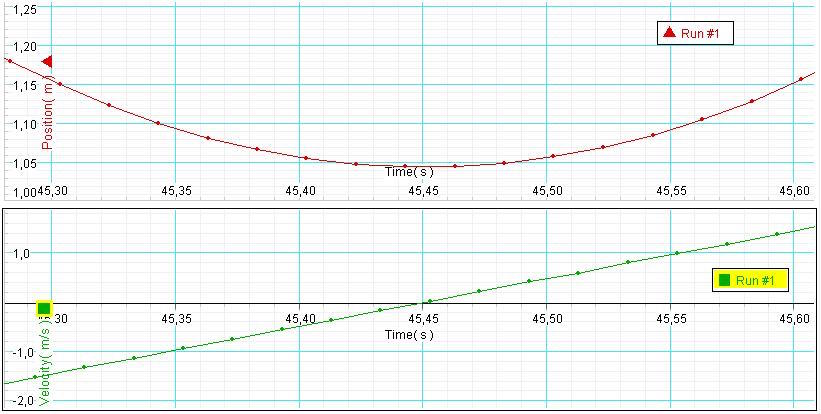
\includegraphics[width=0.9\textwidth]{valbeweging_pasco3}
% \captionof{figure}{Experimenteel bekomen grafieken van een verticale worp}
\end{image}

Als we een appel laten vallen zal de zwaartekracht ervoor zorgen dat de appel naar de aarde valt. Wanneer we bovendien de snelheid meten, zien we dat deze snelheid toeneemt en wel op een constante manier. Dat wil zeggen dat er per tijdseenheid steeds evenveel snelheid bijkomt. De appel valt sneller en sneller maar de mate waarin dat gebeurt, is constant. Gooien we hem op, dan zien we dat zwaartekracht en snelheid tegengesteld zijn aan elkaar. De zwaartekracht zorgt dus duidelijk niet voor de beweging omhoog (de appel blijft omhoog gaan) maar voor een vertraging van de beweging. De snelheid waarmee de appel omhoog beweegt, neemt af. Ook hier zien we -- nadat we meten -- dat de snelheid gelijkmatig afneemt. De snelheid waarmee de appel per tijdseenheid afneemt, is steeds gelijk. Of de appel nu snel gaat of traag, de mate van afname is steeds gelijk. We kunnen dus concluderen dat de zwaartekracht voor een verandering van bewegingstoestand zorgt; de snelheid blijft niet hetzelfde. We zien zelfs dat die verandering van de snelheid gelijkmatig is. De constante zwaartekracht zorgt blijkbaar voor een constante verandering van de snelheid. 

Als je kijkt naar een koppel schoonschaatsers, dan zie je naast een fantastische prestatie en een mooi schouwspel, dat een kracht niet altijd voor een toename of afname in de grootte van de snelheid hoeft te zorgen. 

\begin{image}
% 
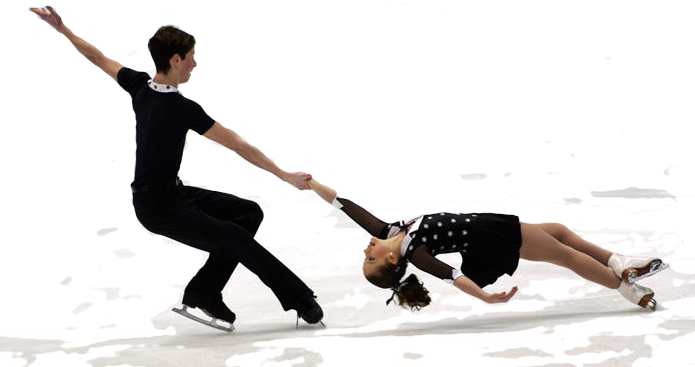
\includegraphics[width=0.7\textwidth]{schoonschaatsers2}
%\captionof{figure}{A gull}
\end{image}

De jongen in de figuur moet duidelijk een kracht uitoefenen om het meisje dat rond hem draait, bij te houden. De kracht die nu wordt uitgeoefend, dient niet zozeer voor het veranderen van de \textit{grootte} van de snelheid dan wel voor het veranderen van de \textit{richting} van de snelheid. Op elk moment verandert de richting van de snelheid, en dit naar de jongen toe -- volgens de richting van de kracht.

We kunnen concluderen dat een kracht niet zozeer invloed uitoefent op de snelheid dan wel op de \textit{verandering} van de snelheid. Deze verandering houdt zowel een verandering van grootte en/of een verandering van richting in. Bovendien blijkt uit de laatste twee voorbeelden dat de verandering te associëren is met de kracht; de verandering is in de richting van de kracht. Snelheid is te beschrijven als een vector en verandering van grootte en/of richting vallen beide onder het veranderen van de vector. Als we die verandering versnelling noemen, lijkt er een relatie te zijn tussen de kracht en de versnelling -- tussen de oorzaak en het gevolg\ldots

In hoofdstuk 1 en 2 bekijken we het formalisme om bewegingen te \textit{beschrijven}. Dit onderdeel noemen we kinematica. In hoofdstuk 3 en 4 behandelen we dan het \textit{verklarende} principe achter de beweging. Dit noemen we dynamica. Het geheel -- kinematica en dynamica -- noemen we mechanica.

\end{document}